 \useunder{\uline}{\ul}{}
\chapter{Team 5 Agent Design}\label{team_6_agent_design}
\section{Introduction}


\section{Social Network}

We don’t want to exclude one’s excellence in one field due to short comes in an irrelevant fields.
Here we have agents’ algorithm for their fight strategy and the algorithm for their leader duties’ functionality potentially written differently. 
Hence, we establish two different trusts, which can decouple an agent’s strategy quality and leadership goodness, 
This does not mean the trusts are completely independent, 
There are still common factors for both of the trusts.
The irrelevant features are excluded from one to another.¬

The agent uses these trusts to summaries features from the left-hand side and contributes to the decision-making of the right-hand side. 

Due to the limited size of the game and size of the features, it is sensible to summaries this 2-d personality based on two trust scores

The boundaries for the trust scores are both at 0.2 and 0.8 and initial scores at 0.5, all of the agents will be True Neutral agents at the beginning and will be the majority for most of the game time. When developing the logic, True Neutral agents are included in all of the interactions, although priority will be given to some other personalities, but 1), the prioritised agents are small amount due to a high standards therefore to make sure there is still the majority of the resource that is left with the bigger amount of agents 2), The accumulated trust addition in a level is less than 0.2 for each of the scores, therefore it will take at least 2 levels for an agent to gain a personality with priority, which ensures enough interaction has happened or enough information is gained for the agent that we can make a new judgment to its personality. When updating the trust, if there is a trust score exceeding the region of 0-1, the max-min scale is applied to all agents. Under this circumstance, there will be at least one min-scored agent and one max-scored agent that has two different personalities that are not neutral. 

\newpage
%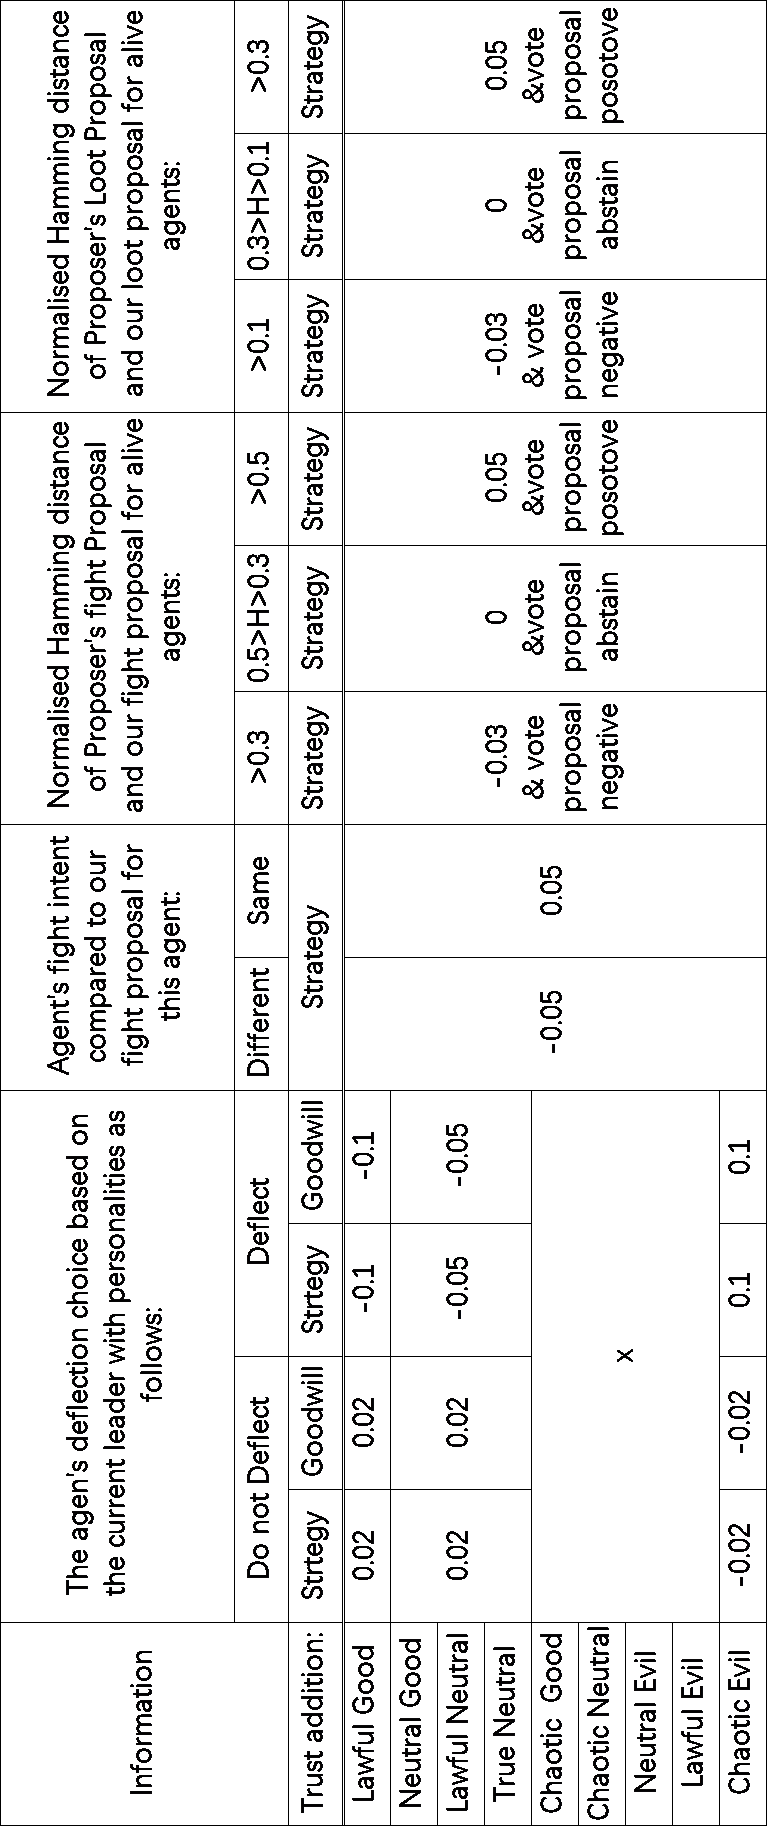
\includegraphics[scale=1]{008_team_5_agent_design/images/Information2Trusts.png}

\begin{SCfigure}[0.5][h]
    \caption{Details of updating trusts regarding different information that can be collected.}
    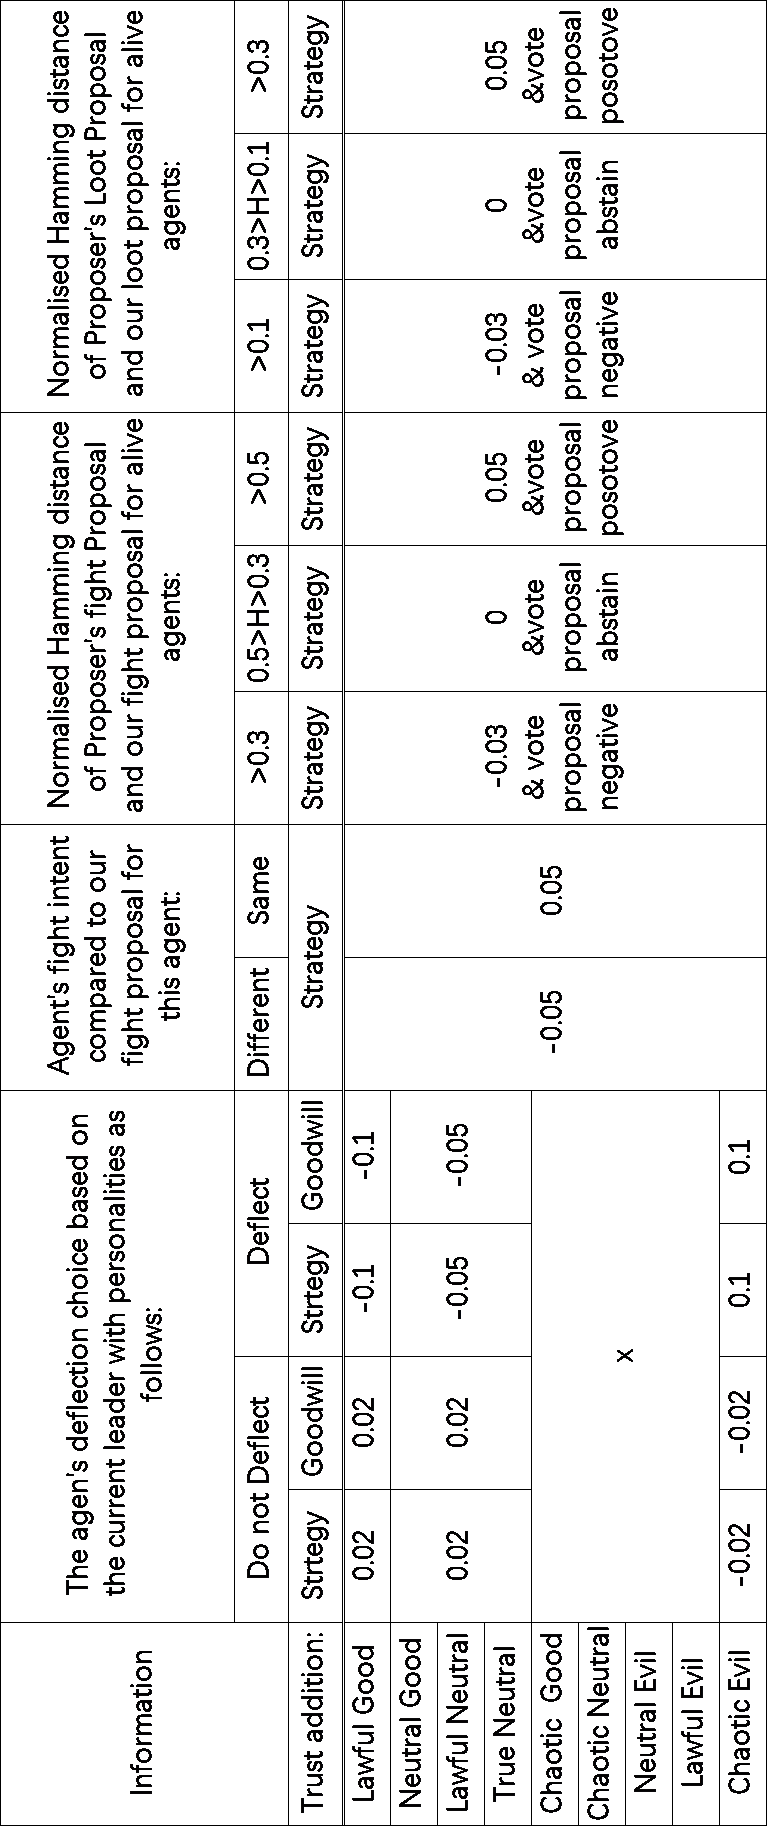
\includegraphics[width=0.63\textwidth]{008_team_5_agent_design/images/Information2Trusts.png}
    \label{fig:Information2Trusts}
\end{SCfigure}
\clearpage

\begin{figure}
    \centering
    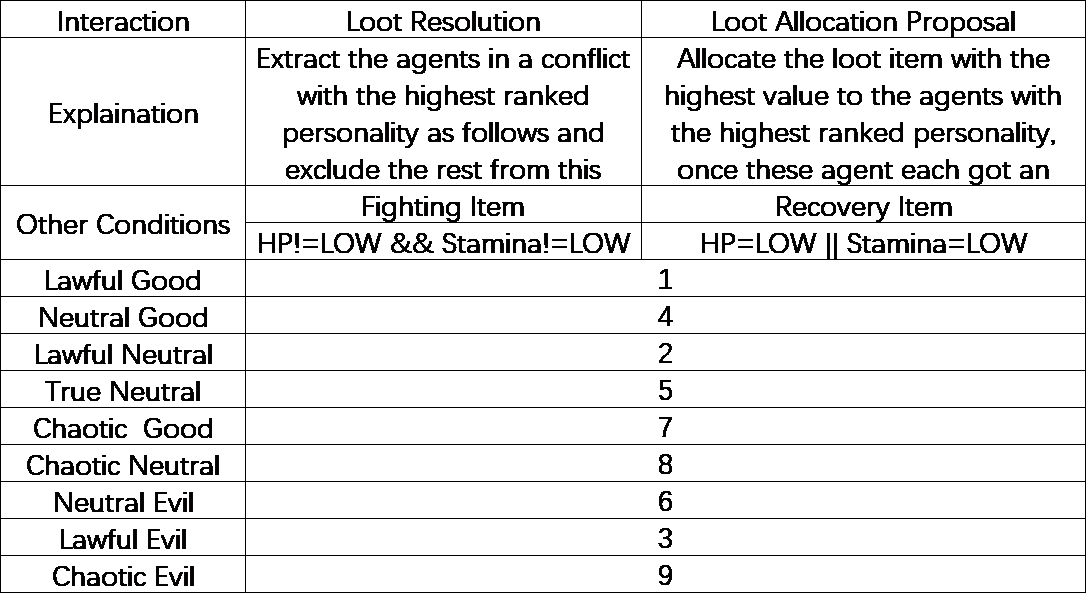
\includegraphics[scale=1]{008_team_5_agent_design/images/Interaction.png}
    \caption{Other agents' personality impact on our agent's interaction behaviour}
    \label{fig:my_label}
\end{figure}


\section{Election}

\section{Leadership Logic}
\subsection{Fight Logic}
\subsection{Loot Allocation}
\subsection{Manifesto}



\section{Fight Logic}



\section{Trading Logic}



\section{Experiment}